\chapter{Prestudy} 
Since the goal of the project is a platform that can increase learning using gamification it was need to conduct a study about which parts of gamification is relevant for the platform and how should they be represented. Peter Parnes, the project owner suggested that the information could be collected by reading literature, having a workshop with teachers at LTU and some teachers outside the university and by interviewing a few teachers teaching in courses that could have use for the platform as a part of their course. An investigation was done about what tools and existing platforms are already available and if they could be reused and built on. This investigation was done by the platform group.

\section{Interviews}
The interviews were done by interviewing a couple of teachers teaching in courses at LTU. A group of four members set up individual meetings with each respective teacher where they asked relevant questions regarding a gamified coding platform. The most comprehensive and general questions during the interviews can be found in appendix~\ref{Interview:questions}. The interview answers from the teachers were summarized to identify the most important elements that could be used. The most important elements were those which were repeated during several interviews and those that the interview group found most interesting. The identified and summarized elements are:

 \begin{itemize}
 \item Mandatory assignments would increase the participation frequency but would be less fun.
 \item Public scoreboard may be demotivating.
 \item Best result could be displayed by a score.
 \item A balance between school and fun.
 \item Levels / different difficulties. 
 \item Even the weaker students should have a chance to solve assignments on the easier levels.
 \item No points or badges.
 \item Anonymous questions.
 \item Good for the lower grades.
 \item Must be easy to adapt the system into a course.
 \end{itemize}
These summarized answers was a good starting point to see which parts should be included later on in the platform and which parts should be excluded. 

\section{Platform}   
To meet the requirements and goals of the project it was clear that a platform that could compile and verify code was needed.
When the project started, the project owner had suggested \techio{} which is a collaborative platform to share coding assignments through open-source ``playgrounds''. At a first glance, the platform seemed to match the needs of the project, but it was unsure if the platform would have an open API which the project communicate and work with. The developers of \techio{}, CodinGame was contacted to find out if they would be open to sharing their API.

%Fyll ut med några av problemen vi identifierade med \techio{} som vi skulle ha behövt lösa om vi hade använt det. (finns i wikin)

While waiting for an answer from \techio{}, an investigation into alternative platforms to \techio{} was launched and after some time of searching for a suitable alternative over the internet it was concluded that no platform found really matched the requirements that were set.

After waiting for several days, \techio{} finally responded where they mentioned the possibility of using ``code snippets'' to embed coding assignments onto other sites than on \techio{}, but they were evasive with the question if they would make their API open and never really answered this. After some time of consideration, a decision to not use \techio{} was made because of the risk of becoming too dependent on their platform.

Because of this, creating a code verification platform/API from scratch was considered. While discussing about making a code verification platform from scratch, a new alternative was brought into light. A computer science student at LTU was currently creating a platform named \sockr{} for code verification and once again, it was considered to use a third party platform.

After some discussions with the student, he explained that he would be open for the project to use \sockr{}. A thorough investigation of the \sockr{} source code was however needed to make sure that it was actually useful for the project. When diving deeper into the source code of \sockr{} it became clear that once again, the project would not be able to use this in a good and sustainable way. While \sockr{} did have the functionality that the project needed, the source code was mostly undocumented, didn't have a clear API and the backend and frontend were too tightly coupled to be used in a sustainable way.

As such, after much research it was concluded that the best and most sustainable thing for the project would be to develop a code verification/compilation platform from scratch, effectively making the project completely independent of other services.


\section{Theory} 
A theory study was conducted where the task was to find what articles and the books have learned about gamification. A group with a couple of members sat down and read books and articles mostly found on internet. The group found a number of useful elements from gamification theory that could possibly be implemented into the platform, it was however realized that not all these elements could be implemented all at once and it was later needed to identify which elements who would gain priority. The elements that the theory group found useful were:
\begin{itemize}
\item Reward
\begin{itemize}
 \item Reward should give positive information since it increases the motivation.
 \item Rewards of controlling type is demotivating.
 \item If rewards ends it may be demotivating later on.
 \item Customization, collect points and be able to spend them.
 \end{itemize}
\item Progress
\begin{itemize}
    \item Progress should be in increasing order.
    \item Be careful with which moments should be graded.
    \item Large numbers are better.
    \item Bonus for overachieving. 
\end{itemize}
\item Freedom
\begin{itemize}
    \item Freely choose between assignments.
    \item Possibility to redo assignments.
\end{itemize}
\item Game mechanics
\begin{itemize}
    \item Chance?
    \item Duels?
    \item Take turns?
\end{itemize}
\item Leaderboard
\begin{itemize}
    \item Anonymous leaderboard.
    \item No disincentive
    \item No ranking, demotivated to have low rank
    \item Populate the leaderboard with fake users
\end{itemize}
\end{itemize}

\section{Comparison interviews and theory} 
To find the key aspects of gamification from both interviews and theory a comparison was made where a group compiled the data from the previous received feedback and other notes collected into a new list that could act as a basis for future decisions about gamification.
When compiling the list it was also important to take into account what parts that could actually be implemented during the project and which ones could be possible future work.
The newly formed list contained the following key elements:
\begin{itemize}
\item A lot of small assignments
\begin{itemize}
 \item A lot of structure, easy to understand the feedback.
 \item Levels.
\end{itemize}
\item Progress
\begin{itemize}
 \item Progress in increasing direction.
\end{itemize}
\item Freedom
\begin{itemize}
 \item The mandatory assignments have highest participation but may be demotivating.
 \item Students should have different options to solve a moment.
 \item Deadlines may be demotivating but also sometimes necessary.
 \item Redo an assignment multiple times.
\end{itemize}
\item Rewards
\begin{itemize}
 \item Should act as a positive information about the student skill level.
 \item Rewards should not act as a controlling factor.
 \item Redeemable points, e.g.\ avatars.
\end{itemize}
\item Feedback
\begin{itemize}
 \item Teachers should be able to check if students have understood the assignment or not.
\end{itemize}
\item Leaderboard
\begin{itemize}
 \item Divided opinions about how good leaderboards are.
 \item Anonymous leaderboards.
 \item Fake users so that no one is last.
\end{itemize}
\end{itemize}


\section{Workshop} 
A workshop was presented as an idea from the project owner Parnes as a way to find out how different teachers think that the system would look like and what features they feel should be included. A group of five people started to work by writing different scenarios for the workshop, see appendix~\ref{Worskshop:senarios}. As a preparation for the real workshop, these scenarios were then tested on a few members of the project group where the members were acting as teachers and they had to implement the planned workshop scenarios. This gave the workshop group some thoughts about what could be improved before the ordinary workshop with the teachers. 
The workshop with the teachers was made by splitting the teachers into two different groups and then they had 10--15 minutes to discuss the scenarios in the group and then another 10 minutes for discussions with the other group. 
The first scenario task was to discuss which type of system and elements could be available that would have motivated them as students. In the scenario 2 the groups had to imagine themselves being the examiners of a course and the groups got to discuss which limitations should be done in the system but also once again, how they could motivate their students. During the scenario 3 the task was to focus on embodying the ideas and thoughts from scenario 1 and 2 into an e-tool and how the general design should for said tool look like. A compiled list from both groups together from what was discussed and concluded during the workshop:
\\
Result from scenario 1
\begin{itemize}
\item Let assignments interlink.
\item Be able to choose which assignments should be done.
    \begin{itemize}
    \item Hard to grade, every goal of the course need to be met.
    \item Assignments with similar content.
    \end{itemize}
\item Constructive alignment, how goals, assignments and examination interacts.
\item Early and quick feedback.
\item Formative assessment, continuous feedback.
\item Groups assignments, hide the personal result.
\item AI Avatar that gives feedback.
\item Lot of visualization of the result.
\item Present the purpose of the assignment.
\item Different angle of the design depending on the user which is solving the assignment.
\end{itemize}

Result from scenario 2
\begin{itemize}
\item Not everything in a course should be change at same time.
\begin{itemize}
\item Old assignments could be divided.
\item Shorter feedback loop.
\item old assignments with new context.
\end{itemize}
\item Updating the course introduction is cheap and makes the goals of the course more clear.
\item When the knowledge should be testes.
\begin{itemize}
\item Thoroughly, min/max, median or average.
\item In the end there is a written exam.
\end{itemize}
\item Invoke from elder students.
\item Peer-to-peer feedback.
\item Test one implementation even if it's bad.
\item Students creates assignments to each other.
\end{itemize}

Result from scenario 3
\begin{itemize}
\item Anonymous questions live
\begin{itemize}
\item ``Did you understand what I said?''
\item Directly feedback.
\end{itemize}
\item Direct chat, students and teacher.
\item Auto generated feedback to the teacher.
\begin{itemize}
\item Aggregate data from relevant measurements.
\end{itemize}
\item A student knowledge bank.
\begin{itemize}
\item Wiki.
\end{itemize}
\item Code correction / evaluation.
\end{itemize}


\begin{figure}[H]
  \centering
  \begin{minipage}[b]{0.7\textwidth}
    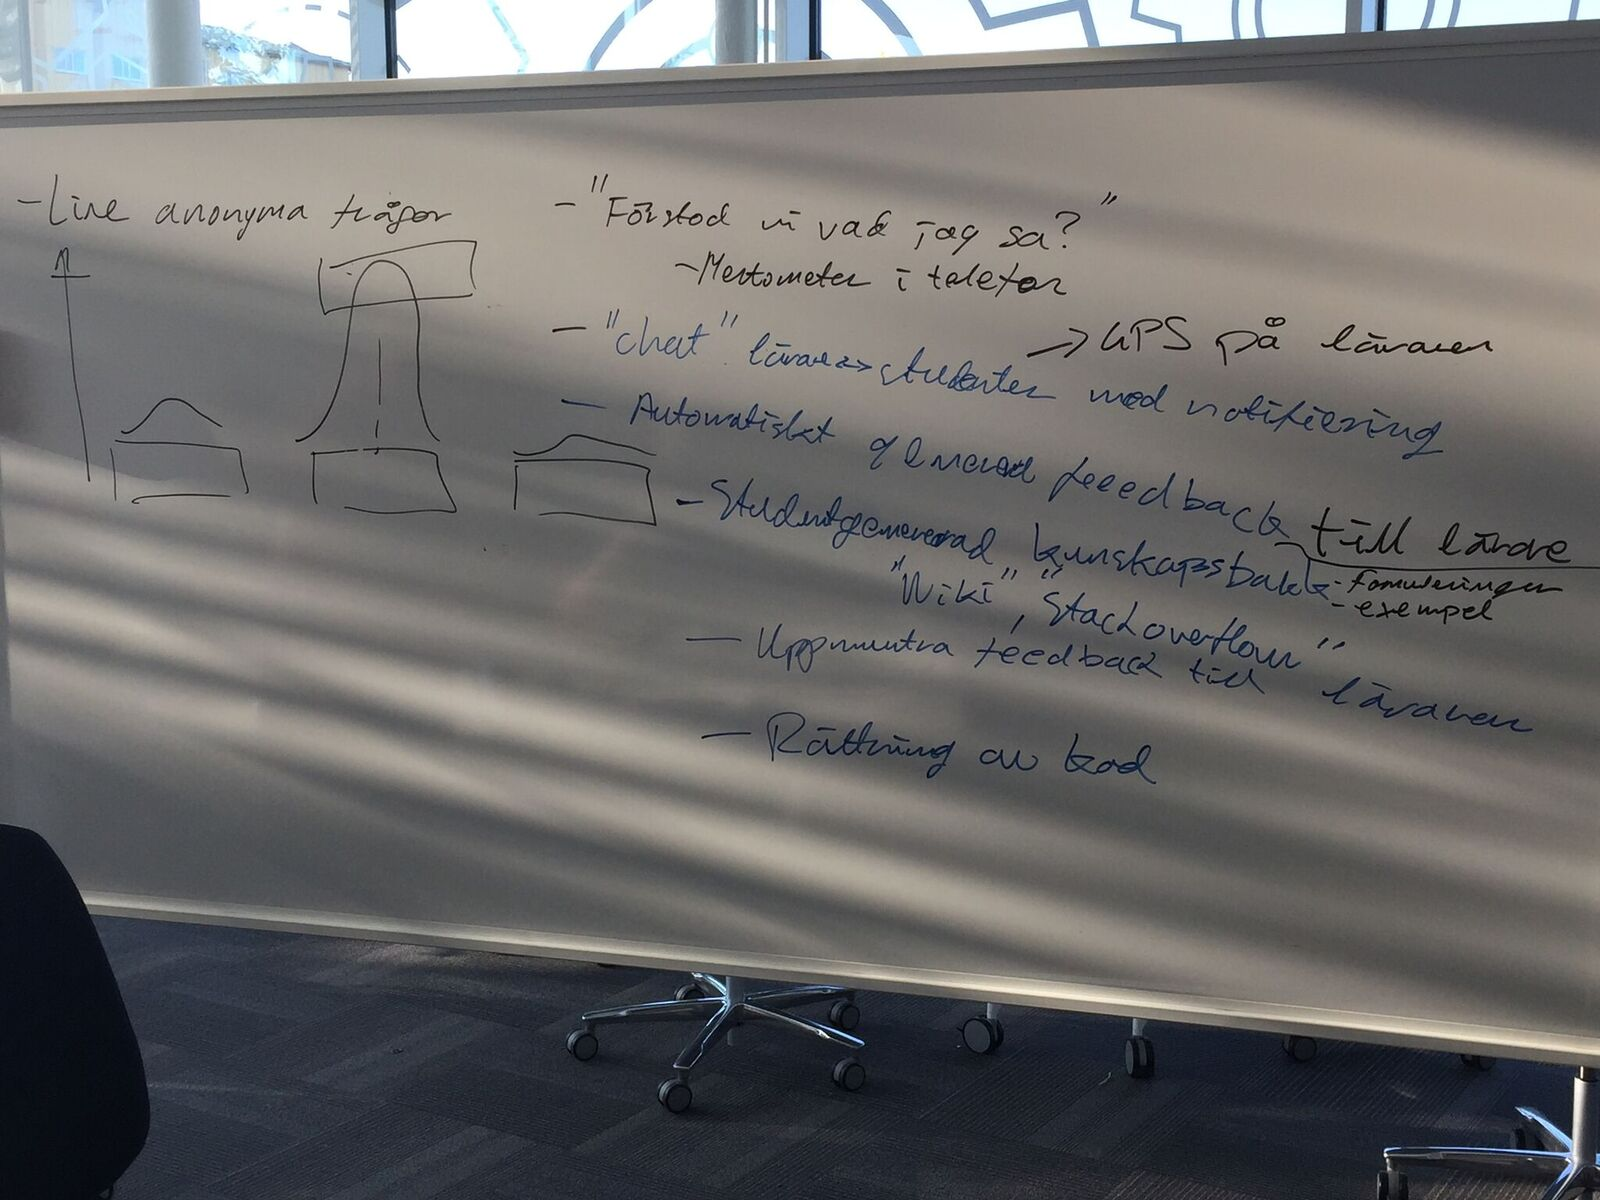
\includegraphics[width=\textwidth]{img/Grupp1_Workshop_mockup.jpg}
    \caption{A mockup over interface from workshop-group 1.}
  \end{minipage}
  \hfill
  \begin{minipage}[b]{0.7\textwidth}
      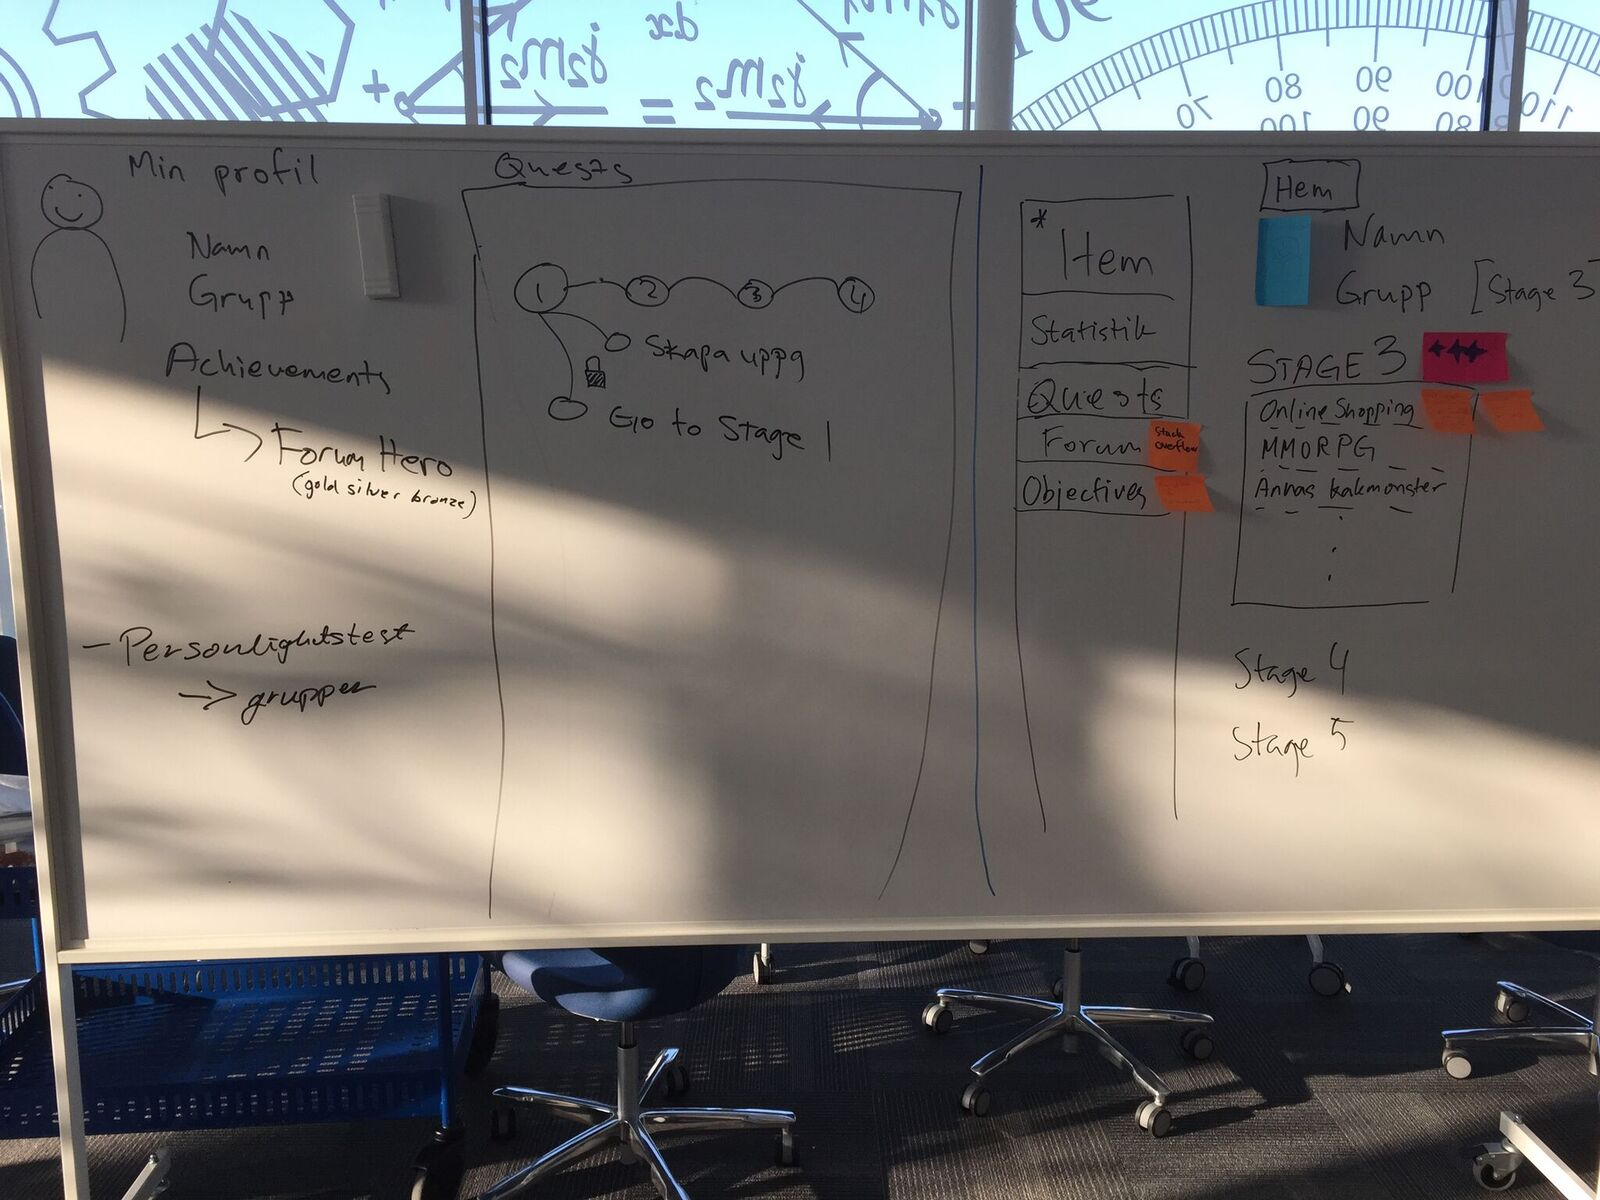
\includegraphics[width=\textwidth]{img/Grupp2_Workshop_mockup.jpg}
    \caption{A mockup over interface from workshop-group 2.}
  \end{minipage}
\end{figure}
